\documentclass[HS.tex]{subfiles}

\begin{document}


%\hyphenation{equi-va-len-cia}\hyphenation{pro-pie-dad}\hyphenation{res-pec-ti-va-men-te}\hyphenation{sub-es-pa-cio}

\chapter{Complejos simpliciales}

\section{Definiciones básicas}

\begin{defi}
Dados los puntos $a_0,\dots, a_n\in\R^n$ afínmente independientes, se define el \emph{$n$-símplice} generado por ellos 
$$\sigma=(a_0,\dots, a_n):=\{x\in\R^n\mid x=\sum_{i=0}^n\lambda_ia_i, \sum_{i=0}^n\lambda_i=1,\lambda_i\geq 0\}.$$
Al número $n$ se le llama \emph{dimensión} del símplice.
\end{defi}

\begin{ej}\
\begin{enumerate}
\item $n=0$: punto, 0-símplice o vértice $(a_0)$.
\item $n=1$: segmento, 1-símplice o arista $(a_0a_1)$.
\item $n=2$: triángulo o 2-símplice   $(a_0a_1a_2)$.
\item $n=3$: tetraedro o 3-símplice $(a_0a_1a_2a_3)$.
\end{enumerate}
\end{ej}

\begin{nota}
Todo $n$-símplice es convexo, pues es la envolvente convexa de los puntos que lo generan. Además es compacto de $\R^n$.
\end{nota}

\begin{defi}
Dado un $n$-símplice $\sigma=(a_0,\dots,a_n)$, se llama \emph{cara} de $\sigma$, y se denota $\tau\leq \sigma$, a cualquier $k$-símplice ($k\leq n$) generado por $k+1$ vértices de $\sigma$. En el caso de que $k<n$ se dirá que $\tau$ es \emph{cara propia} de $\sigma$ y se denotará por $\tau<\sigma$.
\end{defi}

\begin{defi}
Dado el $n$-símplice $\sigma=(a_0,\dots, a_n)$, se define el interior de $\sigma$, denotado por $\mathring{\sigma}$, como
$$\mathring{\sigma}=\{x\in\sigma\mid \lambda_i>0\}.$$
\end{defi}

\begin{ej}\
\begin{enumerate}
\item Para $n=0$, $\sigma=(a_0)$, $\mathring{\sigma}=\sigma$.
\item Para $n=1$, $\sigma=(a_0a_1)$, $\mathring{\sigma}=\sigma-\{a_0,a_1\}$. 
\item Para $n=2$, $\sigma=(a_0a_1a_2)$, $\mathring{\sigma}=\sigma-\{(a_0a_1),(a_1,a_2),(a_0a_2)\}$.
\item Para $n=3$, $\sigma=(a_0a_1a_2a_3)$, $\mathring{\sigma}=\sigma-\{(a_0a_1a_2),(a_0a_1a_3),(a_0a_2a_3),(a_1,a_2a_3)\}$.
\end{enumerate}
\end{ej}

\begin{defi}
Dado un $n$-símplice generado por $\sigma=(a_0,\dots, a_n)$, se define el \emph{borde} de $\sigma$, denotado por $\partial\sigma$, como 
$$\partial\sigma=\bigcup_{\tau<\sigma}\tau.$$
\end{defi}

\begin{prop}
Dado un $n$-símplice $\sigma=(a_0,\dots, a_n)$, se verifica que:
\begin{enumerate}
\item $\sigma=\mathring{\sigma}\sqcup\partial\sigma$.
\item $\mathring{\sigma}=\sigma-\partial\sigma$.
\item $\partial\sigma=\sigma-\mathring{\sigma}$.
\end{enumerate}
\end{prop}

\begin{defi}
Dado $\sigma$ un $n$-símplice, se llama \emph{cara abierta} de $\sigma$ al interior de cualquiera de sus caras.
\end{defi}
\begin{prop}
Todo símplice es unión disjunta de sus caras abiertas.
\end{prop}
\begin{dem}
Sea $x\in\sigma=(a_0,\dots,a_n)\Rightarrow x=\sum_{i=0}^n\lambda_ia_i$ con $\lambda_i\geq 0$ y $\sum_{i=0}^n\lambda_i=1$. Consideramos la cara de $\sigma$ generada por aquellos vértices con $\lambda_i>0$, a cuyo conjunto de índices denotaremos $I=\{i_0,\dots, i_k\}$. Entonce $x=\sum_{i\in I}\lambda_ia_i$, luego $(a_{i_0},\dots,a_{i_k})\leq\sigma$ y contiene a $x$ en su interior. 

Dado que la expresión de $x$ respecto a un sistema de coordenadas es única, esto implica que $(a_{i_0},\dots,a_{i_k})$ es la única cara cuyo interior contiene a $x$.
$\QED$
\end{dem}

\begin{defi}
Un complejo simplicial $K$ en $\R^n$ es una familia de símplices, tales que:
\begin{enumerate}
\item Si $\sigma\in K$ y $\tau\leq\sigma$, $\tau\in K$.
\item Si $\sigma,\sigma'\in K$ tales que $\sigma\cap\sigma'\neq\emptyset$, entonces $\sigma\cap\sigma'\in K$.
\end{enumerate}
\end{defi}

\begin{ej}
\begin{enumerate}
\item Todo $n$-símplice tiene de modo natural estructura de complejo simplicial.
\item Cualquier grafo es un complejo simplicial formado por vértices y aristas.
\item $K=\{(a_0),(a_1),(a_2),(a_0a_1),(a_0a_2),(a_2a_1)\}$.
\item Las triangulaciones de superficies son complejos simpliciales. 
\item Dos aristas que se corten en el interior no lo serían.
\item Un triángulo en el que no estamos incluyendo un vértice dentro de $K$, no lo sería.
\end{enumerate}
\end{ej}\

\begin{defi}
Dado un complejo simpilicial $K$, se define la \emph{realización geométrica} o \emph{poliedro subyacente} de $K$ como el espacio topológico $(|K|,\Tau_e|_{|K|})$ donde $|K|=\underset{\sigma\in K}{\bigcup}\sigma$.
\end{defi}

\begin{defi}
Dado un complejo simplicial $K$ y dado $L\subset K$, si $L$ tiene estructura de complejo simplicial, entonces se dice que $L$ es subcomplejo de $K$.
\end{defi}
\begin{ej}\
\begin{enumerate}
\item Dado un símplice $\sigma$, al considerar todas sus caras propias tenemos un subcomplejo cuya realización es $\partial\sigma$.
\item \underline{El \emph{$p$-esqueleto} de un complejo simplicial $K$}. Se define $\dim(K)=\max\{\dim(\sigma)\mid\sigma\in K\}$. Si $\dim(K)=n$, el $p$-esqueleto de $K$ es el subcomplejo de $K$ dado por
$$K^{(p)}=\{\sigma\in K\mid \dim(\sigma)\leq p\}$$
para $0\leq p\leq n$. Los $p$-esqueletos forman una \emph{filtración}\footnote{\url{https://en.wikipedia.org/wiki/Filtration_(mathematics)}} de $K$. Se deja como ejercicio probar que el $p$-esqueleto es un subcomplejo para todo $0\leq p\leq n$.
\end{enumerate}
\end{ej}

\begin{prop}
Sea $K$ un complejo simplicial finito y $|K|$ su realización geométrica. Entonces $|K|$ es un compacto.
\end{prop}
\begin{dem}
Como todo símplice es compacto y $|K|$ es unión finita de todos sus símplices, entonces $|K|$ es compacto. \QED
\end{dem}

\begin{lemma}
Sea $K$ un complejo simplicial finito, se verifica que $|K|$ es unión disjunta de los interiores de todos sus símplices, es decir, $|K|=\underset{\sigma\in K}\bigsqcup\mathring{\sigma}$.
\end{lemma}
\begin{dem}
$\boxed{\subseteq}$ Dado $x\in |K|$, es claro que existe $\sigma\in K$ tal que $x\in\sigma=(v_0,\dots, v_n)$, pues $|K|=\bigcup_{\sigma\in K}|\sigma|$.  Entonces $x=\sum\lambda_i v_i$. Nos quedamos con los $v_i$ tales que $\lambda_i>0$. De este modo, el símplice $\tau$ generado por dichos vértices es el único de $K$ que contiene a $x$ en su interior. A este símplice lo llamamos \emph{símplice soporte} de $x$. Entonces $x\in\mathring{\tau}\leq \sigma\in K$. Por lo que $x\in \underset{\sigma\in K}\bigsqcup\mathring{\sigma}$.

$\boxed{\supseteq}$ Sea $x\in \underset{\sigma\in K}\bigsqcup\mathring{\sigma}$, entonces existe un único $\sigma\in K$ tal que $x\in\mathring{\sigma}$, luego $x\in |K|$.
\end{dem} 

\begin{defi} Sea $K$ un complejo simplicial y sea $x\in |K|$. Se define la \emph{estrella} de $x$ en $K$ como 
\[
st(x;K)=\{\sigma\in K\mid \exists \tau (\sigma\leq \tau\land x\in\tau)\}.
\]
Esto es, la estrella de $x$ en $K$ la forman todos los símplices de $K$ que contienen a $x$ y todas sus caras.
\end{defi}

\begin{nota}
$st(x;K)$ es un subcomplejo de $K$. Efectivamente, si $\sigma\in st(x;K)$ entonces $\exists \tau$ tal que $\sigma\leq\tau$ y $x\in\tau$. Si $\eta\leq\sigma$, entonces $\eta\leq\tau$, por lo que el mismo $\tau$ para que $\eta\in st(x;K)$. Por otra parte, si $\sigma_1,\sigma_2\in st(x;K)$ y $\sigma_1\cap\sigma_2\neq\emptyset$, entonces $\sigma_1\cap\sigma_2\in K$. Por otra parte, existen $\tau_1,\tau_2\in K$ tales que $x\in\tau_1\cap\tau_2$, y como $\tau_1\cap\tau_2\in K$ y $\sigma_1\cap\sigma_2\leq \tau_1\cap\tau_2$, se tiene que $\sigma_1\cap\sigma_2\in st(x;K)$.
\end{nota}

\begin{defi}
Dado $K$ complejo simplicial y $x\in |K|$, se define el \emph{link} de $x$ en $K$ como
\[
lk(x;K)=\{\sigma\in st(x;K)\mid x\notin\sigma\}.
\]
\end{defi}

\begin{nota}
Análogamente, se tiene que $lk(x;K)$ es subcomplejo tanto de $K$ como de $st(x;K)$. En efecto, si $\sigma\in lk(x;K)$ y $\tau\leq\sigma$ entonces $\tau\in st(x;K)$ y $x\notin \tau$. Además, si $\sigma,\tau\in lk(x;K)$ con $\sigma\cap\tau\neq\emptyset$, entonces $\sigma\cap\tau\in st(x;K)$ y $x\notin\sigma\cap\tau$. 
\end{nota}

\begin{defi}
Sea $K$ un complejo simplicial y sea $\sigma\in K$, se define la \emph{estrella} de $\sigma$ en $K$
\[
st(\sigma;K)=\{\tau\in K\mid \exists\eta\in K (\tau\leq\eta\land \sigma\leq\eta)\}.
\]

Esto es, $st(\sigma;K)$ la forman los símplices que contienen a $\sigma$ como cara y además las caras de dichos símplices.
\end{defi}

\begin{nota}
Se comprueba que cuando $\sigma$ es un vértice, la definición coincide con la estrella del vértice. Además, $st(\sigma;K)$ es subcomplejo de $K$. 
\end{nota}

\begin{defi}
Dado $K$ complejo simplicial y $\sigma\in K$, se define el \emph{link} de $\sigma$ en $K$ como
\[
lk(\sigma;K)=\{\tau\in st(\sigma;k)\mid \sigma\not\leq \tau\}.
\]
También se puede definir equivalentemente como 
\[
lk(\sigma;K)=\{\tau\in st(\sigma;k)\mid \sigma\cap \tau=\emptyset\}.
\]
Se tiene que $lk(\sigma;K)$ es subcomplejo de $K$ y de $st(\sigma;K)$.
\end{defi}

\begin{defi}
Sea $K$ un complejo simplicial y sea $x\in|K|$, se define la \emph{estrella abierta} de $x$ en $|K|$ como
\[
\mathring{st}(x;K)=\bigcup_{x\in\sigma}\mathring{\sigma}
\]
\end{defi}

\begin{prop}
Sea $K$ complejo simplicial y $x\in|K|$, se tiene que
\[
|\mathring{st}(x;K)|=|st(x;K)|-|lk(x;K)|.
\]
\end{prop}
\begin{dem}
$\boxed{\subseteq}$ Sea $y\in |\mathring{st}(x;K)|$. Entonces existe $\sigma\in |K|$ tal que $y\in|\mathring{\sigma}|$, en particular $y\in\sigma$. Como $\sigma\leq\sigma$ y $y\in\sigma$, $y\in |st(x;K)|$. Además, por definición $|lk(x;K)|$ no tiene ningún punto de $|\mathring{st}(x;K)|$, luego $y\notin|\mathring{st}(x;K)|$.

$\boxed{\supseteq}$ Sea $y\in |st(x;K)|-|lk(x;K)|$. Por definición de la estrella, $\exists\eta\in |K|$ tal que $x\in\eta$ y $y\in\eta$. Además, como $y$ no está en el link, $\exists \tau\in |K|$ tal que $y\in\tau$ con $\tau\in |st(x;K)|$ y $x\in\tau$. Consideramos entonces $y\in\tau\cap\eta\in |st(x;K)|$ Como $\tau\cap\eta$ es unión disjunta de sus caras abiertas, entonces, o bien $\tau\cap\eta$ contiene a $y$ en su interior o bien lo contiene alguna de sus caras propias en su interior. En cualquier caso, $y\in |\mathring{st}(x;K)|$.  \QED
\end{dem}

\begin{lemma}
Sea $K$ un complejo simiplicial y sea $A\subseteq|K|$. Se tiene que $A$ es cerrado en $|K|$ si y solo si $A\cap\sigma$ es cerrado de $\sigma$ para todo $\sigma\in K$. 
\end{lemma}
\begin{proof}
$\boxed{\Rightarrow}$ Supongamos que $A$ es cerrado en $|K|$. Por definición de topología relativa, $A\cap\sigma$ es cerrado en $\sigma$ para todo $\sigma\in K$.

$\boxed{\Leftarrow}$. Supongamos que $A\cap\sigma$ es cerrado para todo $\sigma\in K$. Entonces $A=\bigcup_{\sigma\in K} A\cap\sigma$, que como el complejo simplicial es finito, tenemos unión finita de cerrados de $\sigma$. Como $\sigma$ es compacto, tenemos unión finita de compactos, luego $A$ es compacto en $|K|$, luego $A$ es un cerrado.
\end{proof}

El resultado anterior es cierto para abiertos exigiendo que $A\cap\mathring{\sigma}$ sea abierto.

\begin{lemma}
Sea $f:|K|\to X$ donde $K$ es un complejo simplicial y $X$ es un espacio topológico. Entonces $f$ es continua $f|_{\sigma}:\sigma\to X$ es continua para todo $\sigma\in K$.
\end{lemma}
\begin{proof}
 Sea $f:|K|\to X$ es continua, si y solo si para todo $F$ cerrado de $X$ se tiene que $f^{-1}(F)$ es cerrado de $|K|$. Por el lema anterior, esto es equivalente a que $f^{-1}(F)\cap\sigma=f^{-1}|_{\sigma}(F)$ es cerrado, si y solo si $f|_{\sigma}$ es continua.
\end{proof}

\begin{prop}
Dado $K$ complejo simplicial y $x\in|K|$, se tiene que $\mathring{st}(x;K)$ es un abierto de $|K|$ que contiene a $x$ y, en consecuencia, $st(x;K)$ es un entorno de $x$ en $|K|$.
\end{prop}
\begin{dem}
\[
\mathring{st}(x;K)=\bigcup_{x\in \sigma\in K}\mathring{\sigma}.
\]
Basta ver que $\mathring{\sigma}$ es abierto de $|K|$. Veámoslo para el caso de $\sigma=(v_0v_1v_2)$, que será fácilmente generalizable. Sea $\varepsilon=\min\{d_e(y,r_{v_0v_1}),d_e(y,\sigma_{v_0v_2},d_e(y,r_{v_1v_2})\}$, donde $r_{v_iv_j}$ es la recta definida por esos vértices. Como $y\in B_{d_e}(y,\varepsilon/2)\subseteq \mathring{\sigma}$, entonces $\mathring{\sigma}$ es entorno de $y\in\mathring{\sigma}$. Por tanto $\mathring{\sigma}$ es abierto en $|K|$, luego $\mathring{st}(x;K)$ es abierto en $|K|$. 
\QED
\end{dem}

\begin{defi}
Sean $K$ y $K'$ c.s., se dirá que $K'$ es una subdivisión de $K$ si:
\begin{enumerate}
	\item $|K|=|K'|$ como conjuntos.
	\item $\forall σ \in K$ $\exists σ_i' \in K' \mid σ = \bigcup_{i\in I} σ_i'$.
\end{enumerate}
\end{defi}

\begin{ej}
Tenemos el siguiente complejo y una subdivisión suya:

\begin{figure}[H]
\centering
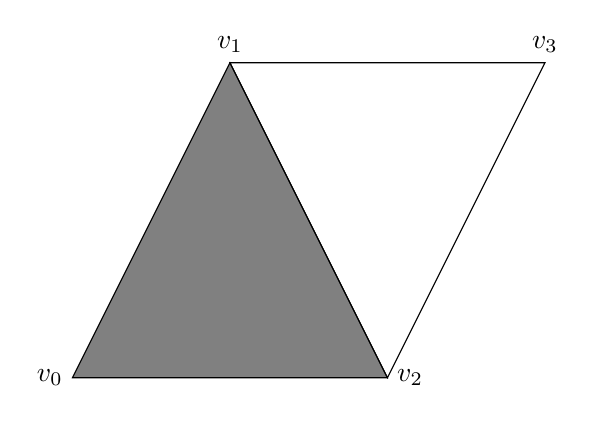
\begin{tikzpicture}
\draw[fill=gray] (0,0) node[anchor=east]{$v_0$} -- (4,0) node[anchor=west]{$v_2$} -- (2,4) node[anchor=south]{$v_1$} -- cycle;
\draw (2,4) -- (4,0) -- (6,4) node[anchor=south]{$v_3$} -- cycle;
\end{tikzpicture}
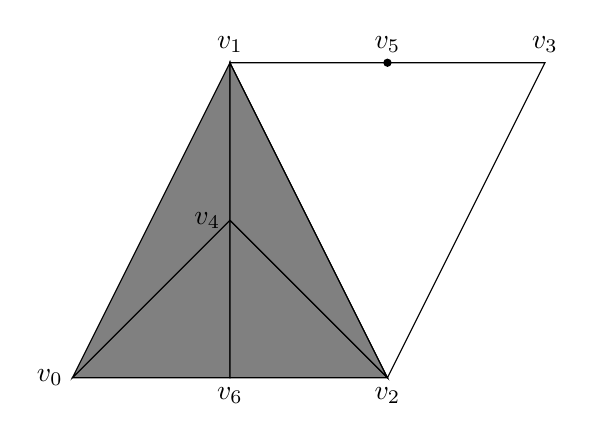
\begin{tikzpicture}
\draw[fill=gray] (0,0) node[anchor=east]{$v_0$} -- (2,0) node[anchor=north]{$v_6$} -- (2,2) node[anchor=west]{$v_4$} -- cycle;
\draw[fill=gray] (0,0) -- (2,2) -- (2,4) node[above]{$v_1$} -- cycle;
\draw[fill=gray] (2,0) -- (2,2) -- (4,0) node[below]{$v_2$} -- cycle;
\draw[fill=gray] (2,2) -- (2,4) -- (4,0) -- cycle;
\draw (2,4) -- (4,0) -- (6,4) node[anchor=south]{$v_3$} -- (4,4) node[anchor=south]{$v_5$} -- cycle;
\draw (2,2) node[anchor=east]{$v_4$};
\fill (4,4)  circle[radius=1.5pt];
\end{tikzpicture}
\end{figure}
\end{ej}

\begin{defi}
Dado el símplice $σ = (v_0,\dots,v_n)$, se define el baricéntro de $σ$ como:
\[ b(σ) = \sum_{i=0}^n \frac{1}{n+1}v_i \]
\end{defi}

\begin{nota}
\begin{enumerate}
\item $b(σ) \in \mathring{σ}$.
\item El baricentro de un vértice es el propio vértice.
\item El baricentro de un $1$-símplice es el punto medio.
\item El baricentro de un $2$-símplice es el baricentro geométrico.
\item Si tenemos una cadena de símplices $σ_1<σ_2<\dots<σ_n$, entonces $b(σ_1),\dots,b(σ_n)$ son afínmente independientes.
\end{enumerate}
\end{nota}

\begin{defi}
Dado un complejo simplicial $K$ se define la primera subdivisión baricéntrica de $K$ como el complejo simplicial $sd K$ formado por todos los símplices del tipo $(b(σ_0),b(σ_1),\dots,b(σ_k))$ donde $σ_0 < σ_1 <\dots <σ_k$ son símplices de $K$.
\end{defi}
\begin{ej}
En la siguiente figura se observa un complejo simplicial y sus baricentros.
\begin{figure}[H]
\centering
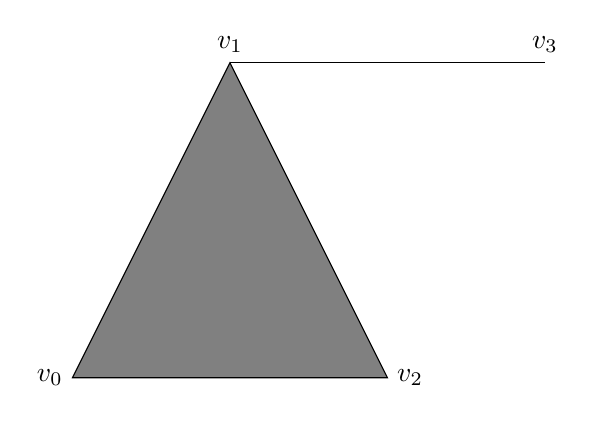
\begin{tikzpicture}
\draw[fill=gray] (0,0) node[anchor=east]{$v_0$} -- (4,0) node[anchor=west]{$v_2$} -- (2,4) node[anchor=south]{$v_1$} -- cycle;
\draw (2,4) -- (6,4) node[anchor=south]{$v_3$};
\end{tikzpicture}
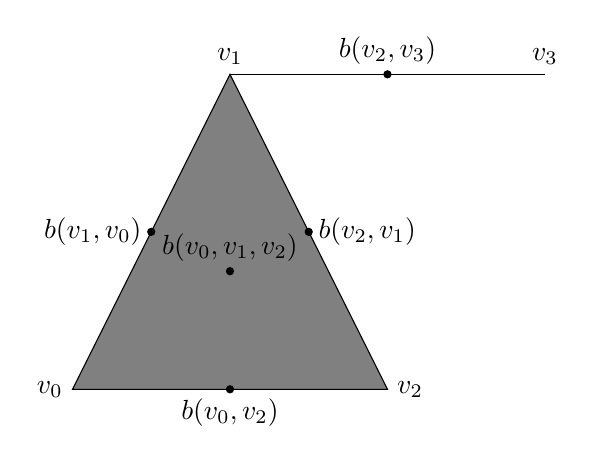
\begin{tikzpicture}
\draw[fill=gray] (0,0) node[anchor=east]{$v_0$} -- (2,0) node[anchor=north]{$b(v_0,v_2)$} -- (4,0) node[anchor=west]{$v_2$} -- (3,2) node[anchor=west]{$b(v_2,v_1)$} -- (2,4) node[anchor=south]{$v_1$} -- (1,2) node[anchor=east]{$b(v_1,v_0)$} -- cycle;
\draw (2,4) -- (4,4) node[anchor=south]{$b(v_2,v_3)$} -- (6,4) node[anchor=south]{$v_3$};
\draw (2,2.1) node[anchor=north]{$b(v_0,v_1,v_2)$};
\fill (3,2)  circle[radius=1.5pt];
\fill (1,2)  circle[radius=1.5pt];
\fill (2,0)  circle[radius=1.5pt];
\fill (2,1.5)  circle[radius=1.5pt];
\fill (4,4)  circle[radius=1.5pt];
\end{tikzpicture}
\end{figure}
\end{ej}

\begin{prop}
$sd K$ es una subdivisón de $K$.
\end{prop}
\begin{dem}
\begin{enumerate}
\item Veamos que $|K|=|sd K|$ por doble inclusión.
Sea $x \in |sdK|$, entonces existe $σ \in sd K$ tal que $x \in σ$, luego $x \in |K|$.
Sea $x \in |K|$, sea $σ$ el soporte de $x$ en $K$ y calculamos $b(σ)$. (Seguimos en la siguiente clase) \QED
\end{enumerate}
\end{dem}

\end{document}